\documentclass[notheorems,mathserif,table,compress]{beamer}  %dvipdfm选项是关键,否则编译统统通不过
%%------------------------常用宏包------------------------
%%注意, beamer 会默认使用下列宏包: amsthm, graphicx, hyperref, color, xcolor, 等等
\usepackage{fontspec,xunicode,xltxtra}
\usepackage{amsfonts,amssymb}  % for XeTeX
%%------------------------ThemeColorFont------------------------
%% Presentation Themes
% \usetheme[<options>]{<name list>}
\usetheme{Madrid}
%% Inner Themes
% \useinnertheme[<options>]{<name>}
%% Outer Themes
% \useoutertheme[<options>]{<name>}
\useoutertheme{miniframes} 
%% Color Themes 
% \usecolortheme[<options>]{<name list>}
%% Font Themes
% \usefonttheme[<options>]{<name>}
\setbeamertemplate{background canvas}[vertical shading][bottom=white,top=structure.fg!7] %%背景色, 上25%的蓝, 过渡到下白.
\setbeamertemplate{theorems}[numbered]
\setbeamertemplate{navigation symbols}{}   %% 去掉页面下方默认的导航条.
\usepackage{zhfontcfg}
\usepackage{iplouclistings}
\usepackage{fancybox}
\usepackage{latexsym}
\usepackage{xcolor}
\usepackage{subfigure} %%图形或表格并排排列
\usepackage{tcolorbox}
%%自己加宏包
\usepackage{pifont}
\usepackage[perpage,symbol*]{footmisc}
\usepackage{multirow}


\newcommand\zhyfly[2][purple]{\hskip5pt\shadowbox{\color{#1}\small\lishu #2\vspace{2mm}}}
%\setsansfont[Mapping=tex-text]{文泉驿正黑}  %% 需要fontspec宏包
     %如果装了Adobe Acrobat,可在font.conf中配置Adobe字体的路径以使用其中文字体
     %也可直接使用系统中的中文字体如SimSun,SimHei,微软雅黑 等
     %原来beamer用的字体是sans family;注意Mapping的大小写,不能写错
     %设置字体时也可以直接用字体名,以下三种方式等同:
     %\setromanfont[BoldFont={黑体}]{宋体}
     %\setromanfont[BoldFont={SimHei}]{SimSun}
     %\setromanfont[BoldFont={"[simhei.ttf]"}]{"[simsun.ttc]"}
%%------------------------MISC------------------------
\graphicspath{{figures/}}         %% 图片路径. 本文的图片都放在这个文件夹里了.
%%------------------------正文------------------------
\begin{document}
\XeTeXlinebreaklocale "zh"         % 表示用中文的断行
\XeTeXlinebreakskip = 0pt plus 1pt % 多一点调整的空间
%%----------------------------------------------------------
%% This is only inserted into the PDF information catalog. Can be left
%% out.
%%%
%% Delete this, if you do not want the table of contents to pop up at
%% the beginning of each subsection:
\AtBeginSection[]{                              % 在每个Section前都会加入的Frame
  \frame<handout:0>{
    \frametitle{内容提要}\small
    \tableofcontents[current,currentsubsection]
  }
}
\AtBeginSubsection[]                            % 在每个子段落之前
{
  \frame<handout:0>                             % handout:0 表示只在手稿中出现
  {
    \frametitle{下一节内容}\small
    \tableofcontents[current,currentsubsection] % 显示在目录中加亮的当前章节
  }
}
%%----------------------------------------------------------
\title[	垂测电离图E区描迹自动判读方法]{基于图像处理的垂测电离图E区描迹自动判读方法}
%\subtitle{Mathematics of Scientific Computing}
\author[孙晓庆]{姓~~名~~~~~\textcolor{olive}{孙晓庆}\\
    导~~师~~~~~\textcolor{olive}{郑海永} \\~~~~~~~~~~~~专~~业~~~~~\textcolor{olive}{电子与通信工程}}
\institute[中国海洋大学]{\kaishu\small\textcolor{violet}{中国海洋大学~~信息科学与工程学院}}
\date{2016~年~5~月~22~日}
\titlegraphic{

\includegraphics[height=2cm]{ouc-logo.png}}
%\titlegraphic{\vspace{-6em}\includegraphics[height=7cm]{ouc}\vspace{-6em}}
\frame{ \titlepage }
%%----------------------------------------------------------
\section*{目录}
\frame{\frametitle{目录}\tableofcontents}
%%============================================================================================================================
\section{选题背景及国内外研究现状}
%\subsection{选题背景及意义}%如果你想书签不出现问题,请不要用\XeTeX
 
%-----------------------------------------------------------------------------------------------------------------------------
%\begin{frame}
%  \frametitle{视觉注意}
%\begin{figure}[!htb] %插图
%\centering
%\includegraphics[width=0.9\textwidth]{network1.png}
%\caption{互联网用户上传数千亿幅照片}
%\label{fig:1}
%\end{figure}
  % \XeTeXpicfile "./logo.jpg" xscaled 100 yscaled 100 %插图也没有问题
%\end{frame}

%-----------------------------------------------------------------------------------------------------------------------------
\begin{frame}
  \frametitle{选题背景}
  \begin{itemize}
  \item  {\color{blue}{电离层}}是受太阳高能辐射和宇宙线的激励而电离的大气高层(离地面约60km~1000km)。
  \item 电离层影响广播电视通信、GPS导航、国防雷达监测、地震预测。
  \end{itemize}
\begin{figure}[!htb] %插图
\centering
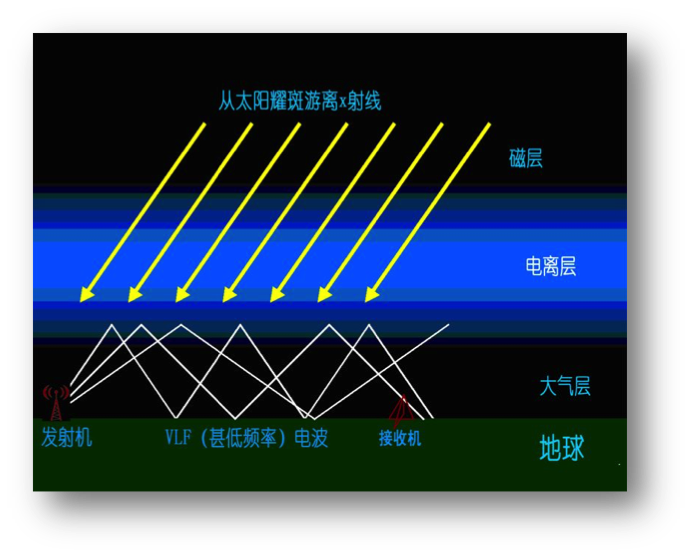
\includegraphics[width=0.5\textwidth]{电离图.png}
%\caption{互联网用户上传数千亿幅照片}
\label{fig:2}
\end{figure}
  % \XeTeXpicfile "./logo.jpg" xscaled 100 yscaled 100 %插图也没有问题
\end{frame}

%-----------------------------------------------------------------------------------------------------------------------------
\begin{frame}
  \frametitle{选题背景}
 {\color{blue}{垂直探测原理:}}
 %通过地面的测高仪垂直向高空发射频率随时间变化的无线电脉冲,在同一地点接收这些脉冲的电离层反射信号,
 探测仪通过记录发射和接收脉冲之间的时间延迟,获取电离层的高度信息(虚高)。\\
{\color{blue}{垂测电离图:}}虚高随发射频率变化的曲线图。
\begin{figure}[!htb] %插图
\centering
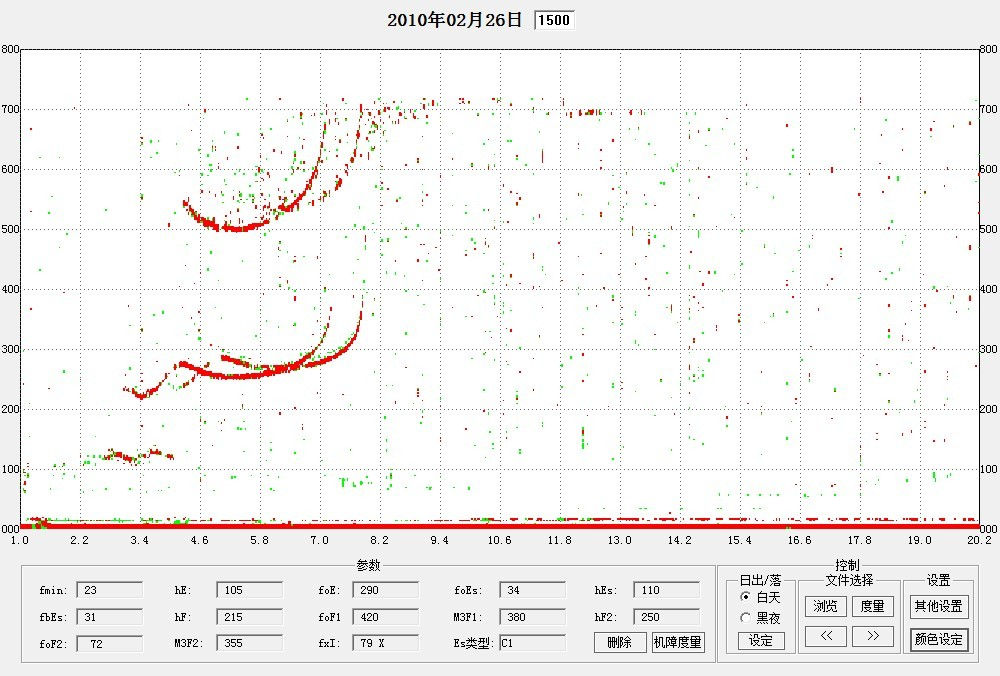
\includegraphics[width=0.55\textwidth]{ManualIonogram.png}
%\caption{互联网用户上传数千亿幅照片}
\label{fig:2}
\end{figure}
  % \XeTeXpicfile "./logo.jpg" xscaled 100 yscaled 100 %插图也没有问题
\end{frame}

\begin{frame}
  \frametitle{选题背景}
    \begin{itemize}
      \item 测高仪及其得到的电离图数量逐年增长;
      \item 电离图人工判读费时、费力且存在主观因素差异。
        \end{itemize}
  \end{frame}
  
  \begin{frame}
  \frametitle{国内外研究现状}
    \begin{itemize}
      \item[]国外研究进展:\\
           \begin{itemize}
           \item 美国UMLCAR提出了ARTIST方法(曲线拟合、人工神经网络)
            \item 意大利INGV提出了Autoscala方法 (相关技术)  
            \item 美国SEC提出了ERSI方法 (物理模型)
            \end{itemize}
      \item[]国内研究进展:
          \begin{itemize}
          \item 中科院的宁百齐、丁宗华等(经验正交分解)
          \item 中国电波传播研究所 (模型反演、描迹检索)
            \end{itemize}
         \item[] {\color{blue}{依赖于探测方式及探测仪,对电离图E区描迹的自动判读研究较少}}。
        \end{itemize}
     
  \end{frame}

%=============================================================================================================================
\section{主要研究内容及总体流程图}
%\subsection{4.6.1 Basic Concepts}%如果你想书签不出现问题,请不要用\XeTeX
                                 %这类复杂的指令,直接写XeTeX吧
\begin{frame}
  \frametitle{主要研究内容}
   \begin{itemize}
  \item 自动提取并识别电离图E区描迹;
  \item 自动获取电离图E区参数$foE$、$h'E$、$foEs$、$fbEs$、$h'Es$、$Es$类型。
  \end{itemize}
  
  
  
  
 \begin{figure}[!htb] %插图
\centering
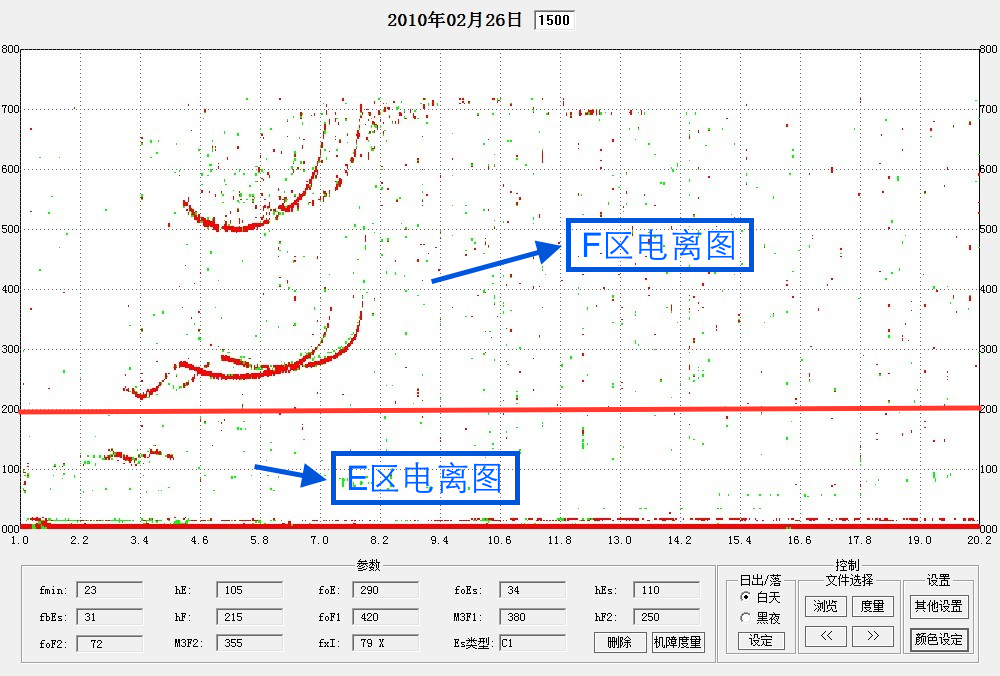
\includegraphics[width=0.55\textwidth]{分割图例.png}
%\caption{互联网用户上传数千亿幅照片}
\label{fig:2}
\end{figure}
\end{frame}


 
  \begin{frame}
\frametitle{课题难点及思路}
\color{blue}\textbf{电离图E区描迹主要特点:}
\begin{itemize}
\item [] 类型多样性(11种Es层类型描迹)
\item [] 描迹形态多样性
\item [] 描迹的扩散现象
\item [] 出现没有规律性
\end{itemize}
\pause
\color{blue}\textbf{研究思路:人工度量经验+图像处理技术}
\begin{itemize}
\item [] \textbf{人是如何度量电离图}$\Rightarrow$系统架构
\item [] \textbf{图像处理与图像分析}$\Rightarrow$算法设计
\end{itemize}
%\pause
%\color{blue}\textbf{研究准备:}
%\begin{itemize}
%\item [] 构建数据集
%\item [] 学习人工度量知识
%\item [] 总结人工度量经验
%\end{itemize}
\end{frame}

 
\begin{frame}
 \frametitle{总体算法流程图}
\begin{center}
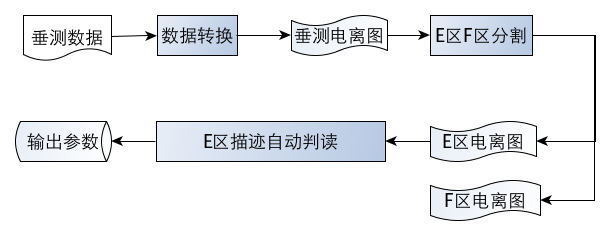
\includegraphics[width=0.9\linewidth]{总体流程图.png}%
\end{center}
\end{frame}

%-----------------------------------------------------------------------------------------------------------------------------
%\begin{frame}
%  \frametitle{预处理}
%\begin{itemize}
%\item RGB彩色模型;
%\item Lab 彩色模型;
%\item IRGBY 彩色模型;
%\item 图像尺度调整模型;
%\end{itemize}
%\pause
%\end{frame}

%-----------------------------------------------------------------------------------------------------------------------------
%\begin{frame}
%  \frametitle{时频变换}
%\begin{itemize}
%\item 傅里叶变换;
%\item 离散余弦变换;
%\item 小波变换;
%\item 四元数傅里叶变换;
%\end{itemize}
%\pause
%\end{frame}

%=============================================================================================================================
%\section{频域显著性检测模型}
%-----------------------------------------------------------------------------------------------------------------------------
%\pause
\section{本文主要工作}
\subsection{电离图E区F区分割}
\begin{frame}
 \frametitle{电离图E区F区分割 }
\begin{tcolorbox}[colback=blue!5,colframe=blue!75!black]
\begin{description}
\vspace{-0.5em}
\addtolength{\itemindent}{-4em}
\item[目的] 方便于E区F区描迹的定位、简化后期算法的复杂度
\item[依据] E区F区谷区、E区F区描迹的实际情况
\item[算法] 水平投影积分法+\color{blue}\textbf{人工度量经验}
\vspace{-1em}
\end{description}
\end{tcolorbox}
\begin{figure}[!htb] %插图
\centering
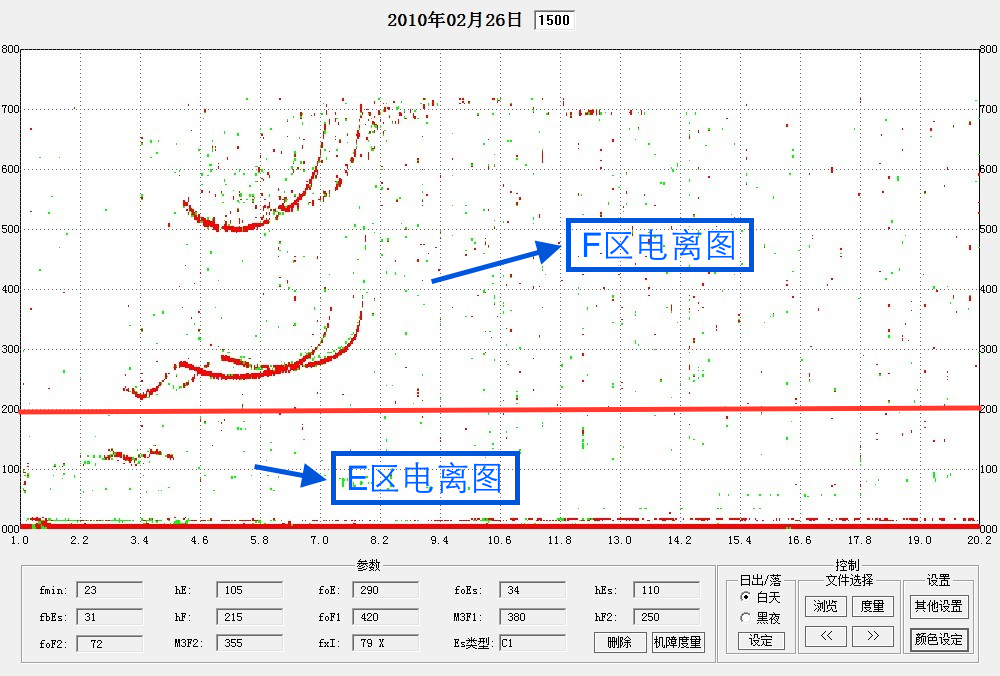
\includegraphics[width=0.55\textwidth]{分割图例.png}
%\caption{互联网用户上传数千亿幅照片}
\label{fig:2}
\end{figure}
\end{frame}

\begin{frame}
 \frametitle{电离图E区F区分割 }
\begin{center}
  \begin{minipage}[t]{0.45\linewidth}  
    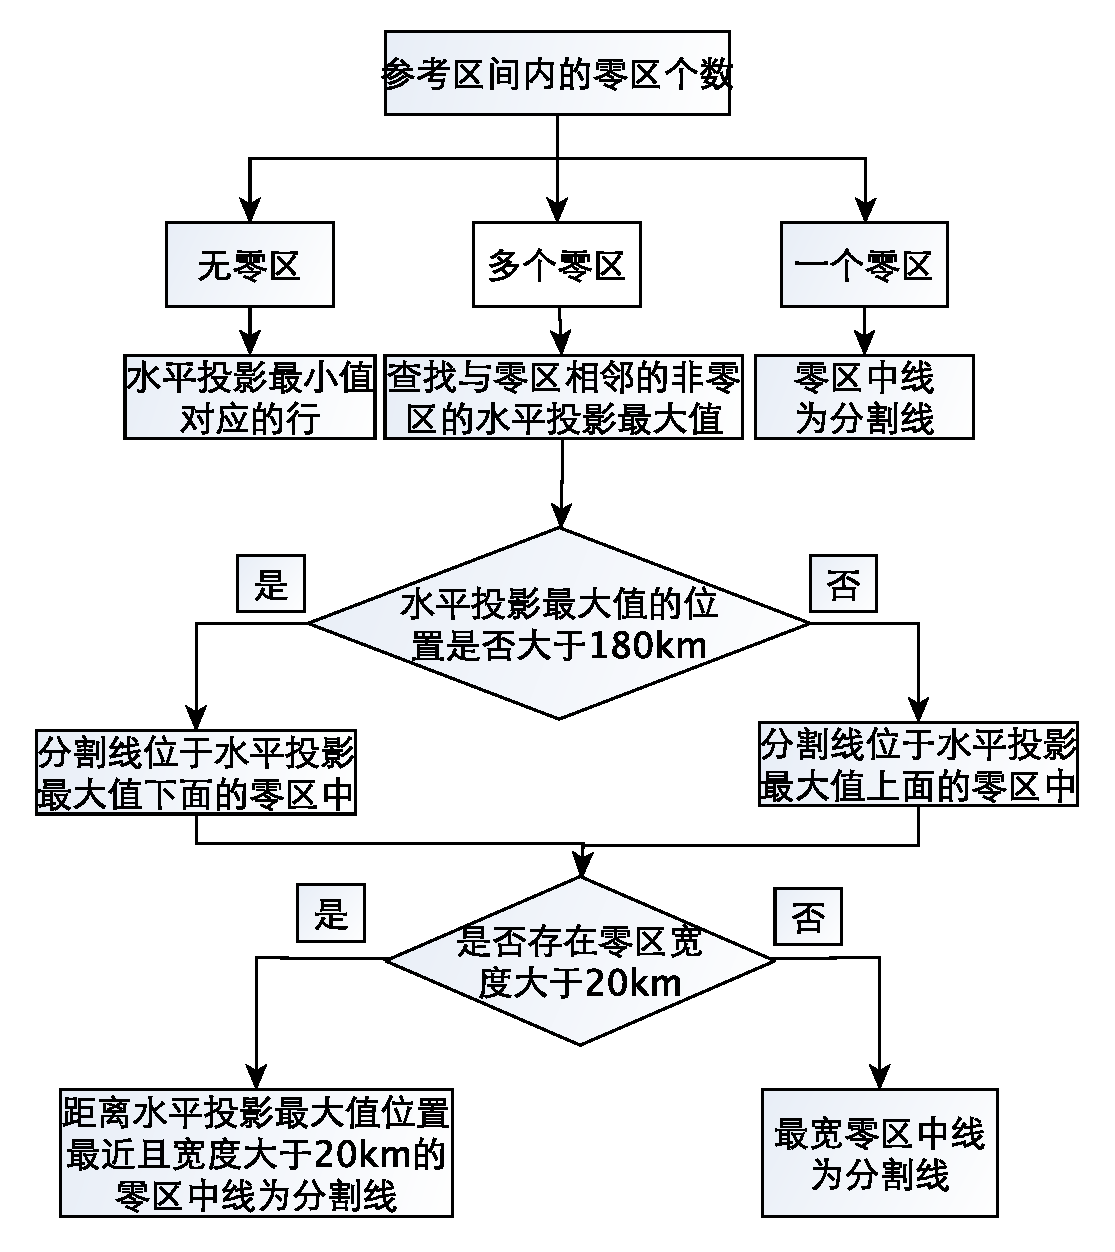
\includegraphics[width=1\linewidth]{newnewE区F区分割方案.pdf} 
  \end{minipage}
  \begin{minipage}[t]{0.5\linewidth} 
    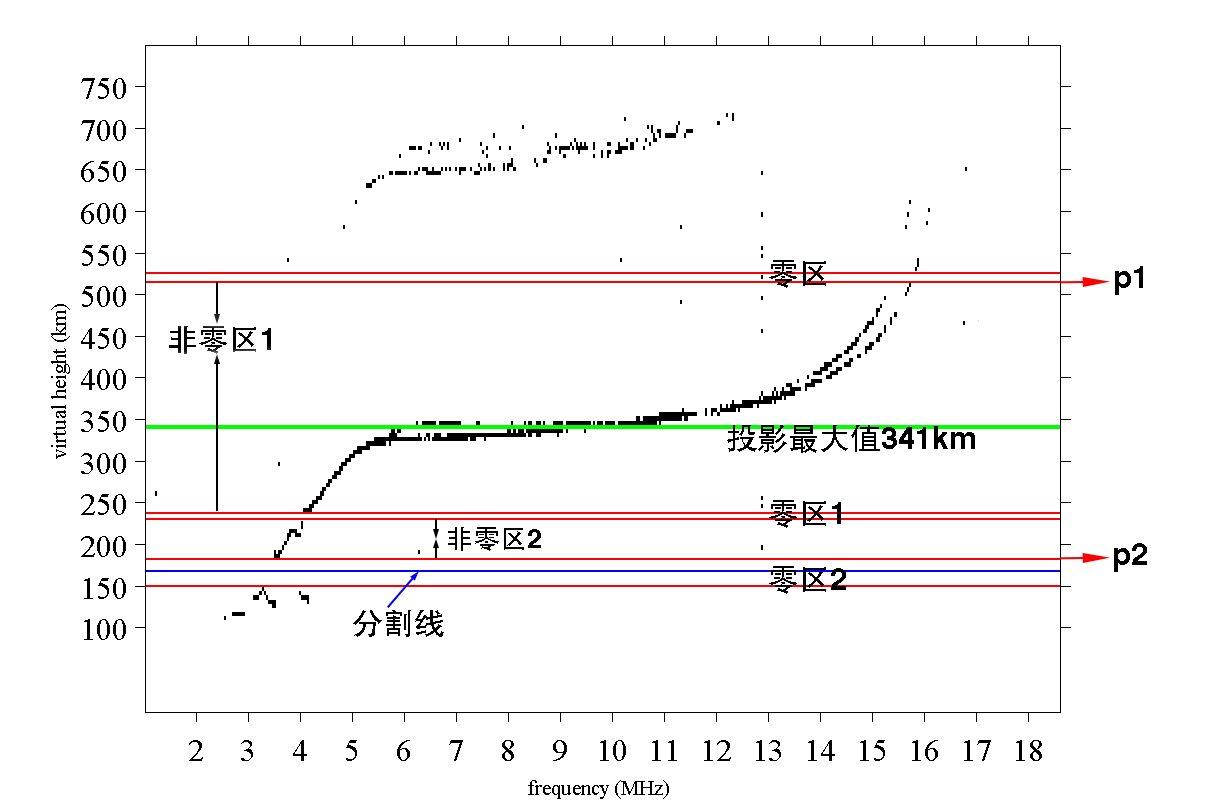
\includegraphics[width=1\linewidth]{201303121545p40s1-EregionExample6.png} 
  \end{minipage}
\end{center}
\end{frame}

%=============================================================================================================================
\subsection{E区电离图类型识别与参数度量}
\begin{frame}
 \begin{figure}[ht!]
    \centering
  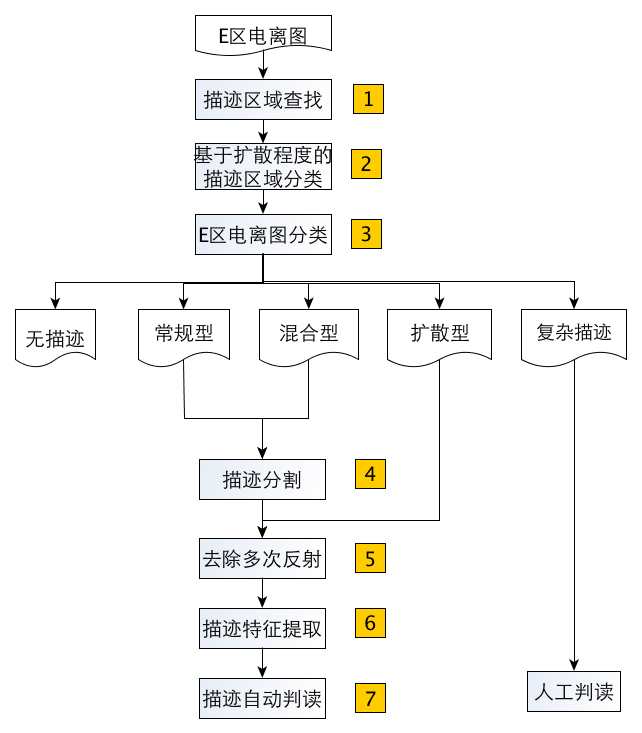
\includegraphics[width=0.55\linewidth]{E区描迹度量方案修改版.png}
 \end{figure}
 
%\begin{center}
%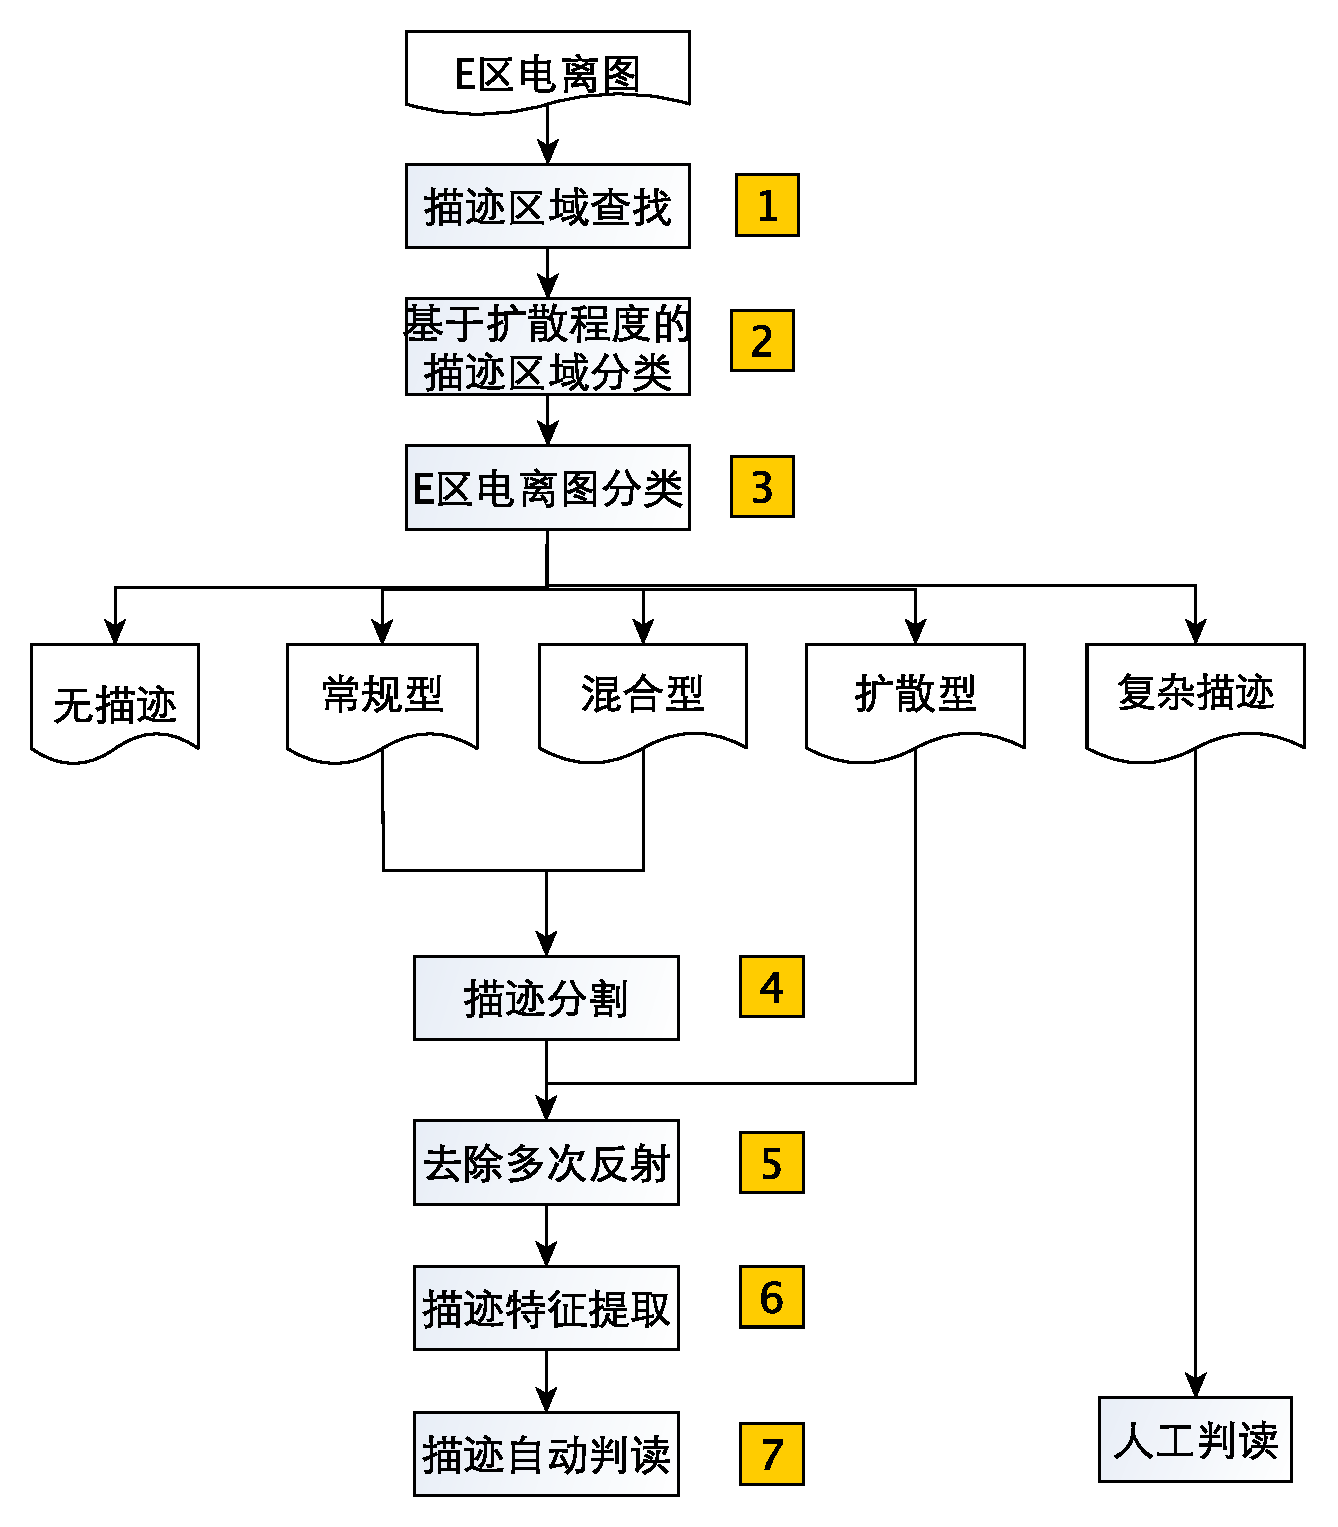
\includegraphics[width=0.55\linewidth]{E区描迹度量方案修改版.pdf}%
%\end{center}
\end{frame}

\begin{frame}
\frametitle{\ding{202} E区描迹区域查找}
\begin{tcolorbox}[colback=blue!5,colframe=blue!75!black]
\begin{description}
\vspace{-0.5em}
\addtolength{\itemindent}{-4em}
\item[目的] 描迹在哪里?
\item[依据] “描迹区域”:电离图上有值像素点(回波信号)较密集的区域
\item[算法] \mbox{}
\begin{enumerate}
\item \textcolor{blue}{\textbf{候选描迹区域查找}}
\item \textcolor{blue}{\textbf{非描迹区域排除}}
\end{enumerate}
\end{description}
\end{tcolorbox}
\end{frame}

\begin{frame}
\frametitle{\ding{72} 候选描迹区域查找}
\begin{tcolorbox}[colback=blue!5,colframe=blue!75!black]
\begin{itemize}
\vspace{-0.5em}
\addtolength{\itemindent}{-2em}
\item 积分图法$\Rightarrow$密集点集
\item 数学形态学$\Rightarrow$候选描迹区域%膨胀、腐蚀、连通区域标记
\vspace{-1em}
\end{itemize}
\end{tcolorbox}
\centering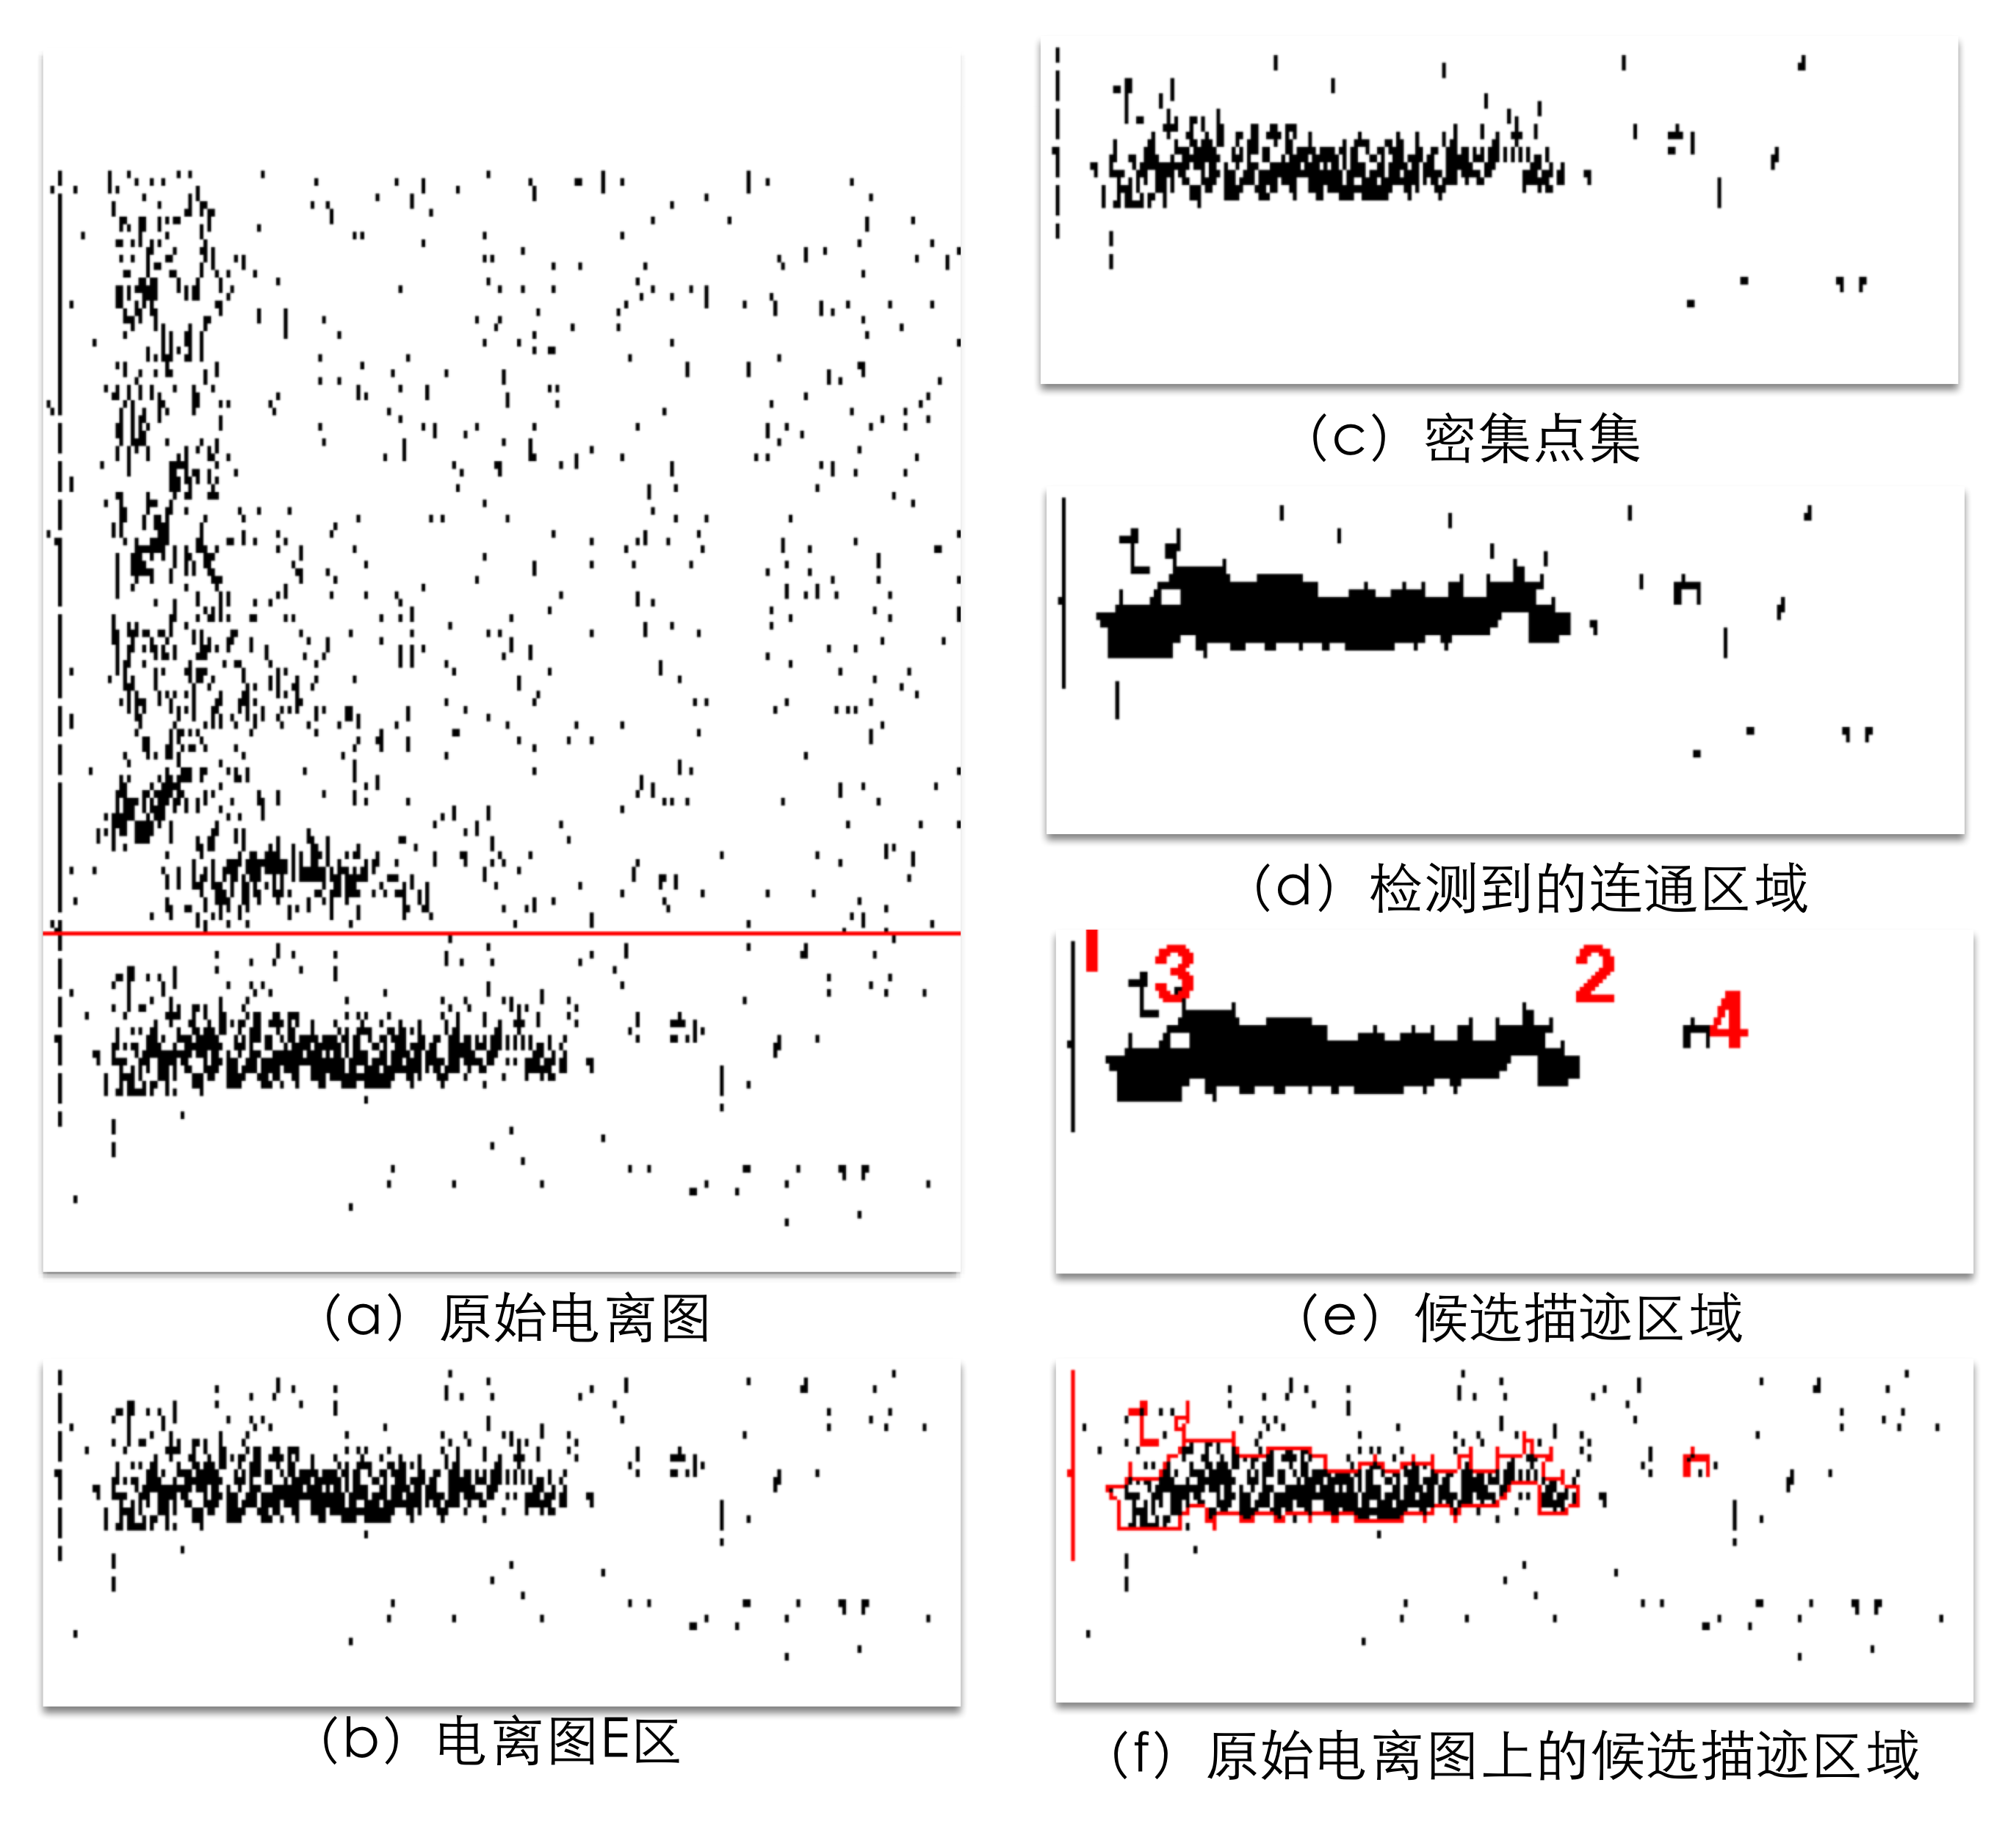
\includegraphics[width=0.55\linewidth]{检测描迹候选区域.png}
\end{frame}

\begin{frame}
\frametitle{\ding{72} 非描迹区域排除}
\begin{tcolorbox}[colback=blue!5,colframe=blue!75!black]
\begin{description}
\vspace{-0.5em}
\addtolength{\itemindent}{-2em}
\item[思路] 视觉特征$\Rightarrow$量化特征
\item[视觉特征] 描迹区域的位置信息、描迹区域的扩散情况、描迹信息、描迹区域的大小
\item[量化特征] 区域像素密度$\rho_{area}$、区域的位置$(x_{\max},y_{\max})$、长度$l_{area}$、宽度$w_{area}$、非零像素点个数$N_{nonzero}$
\vspace{-0.5em}
\end{description}
\end{tcolorbox}
\centering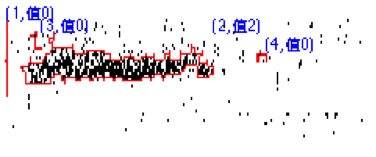
\includegraphics[width=0.7\linewidth]{排除结果.png}
\end{frame}

\begin{frame}
\frametitle{\ding{203} 基于扩散程度的E区描迹区域分类}
\begin{tcolorbox}[colback=blue!5,colframe=blue!75!black]
\begin{description}
\vspace{-0.5em}
\addtolength{\itemindent}{-2em}
\item[目的] 描迹区域内是什么?
\item[依据] 区域内描迹的像素分布特点
\item[扩散密度] 描迹区域\textcolor{blue}{\textbf{扩散密度}}$\rho_{spread}$衡量描迹的扩散程度
\vspace{-0.5em}
\end{description}
\end{tcolorbox}
\centering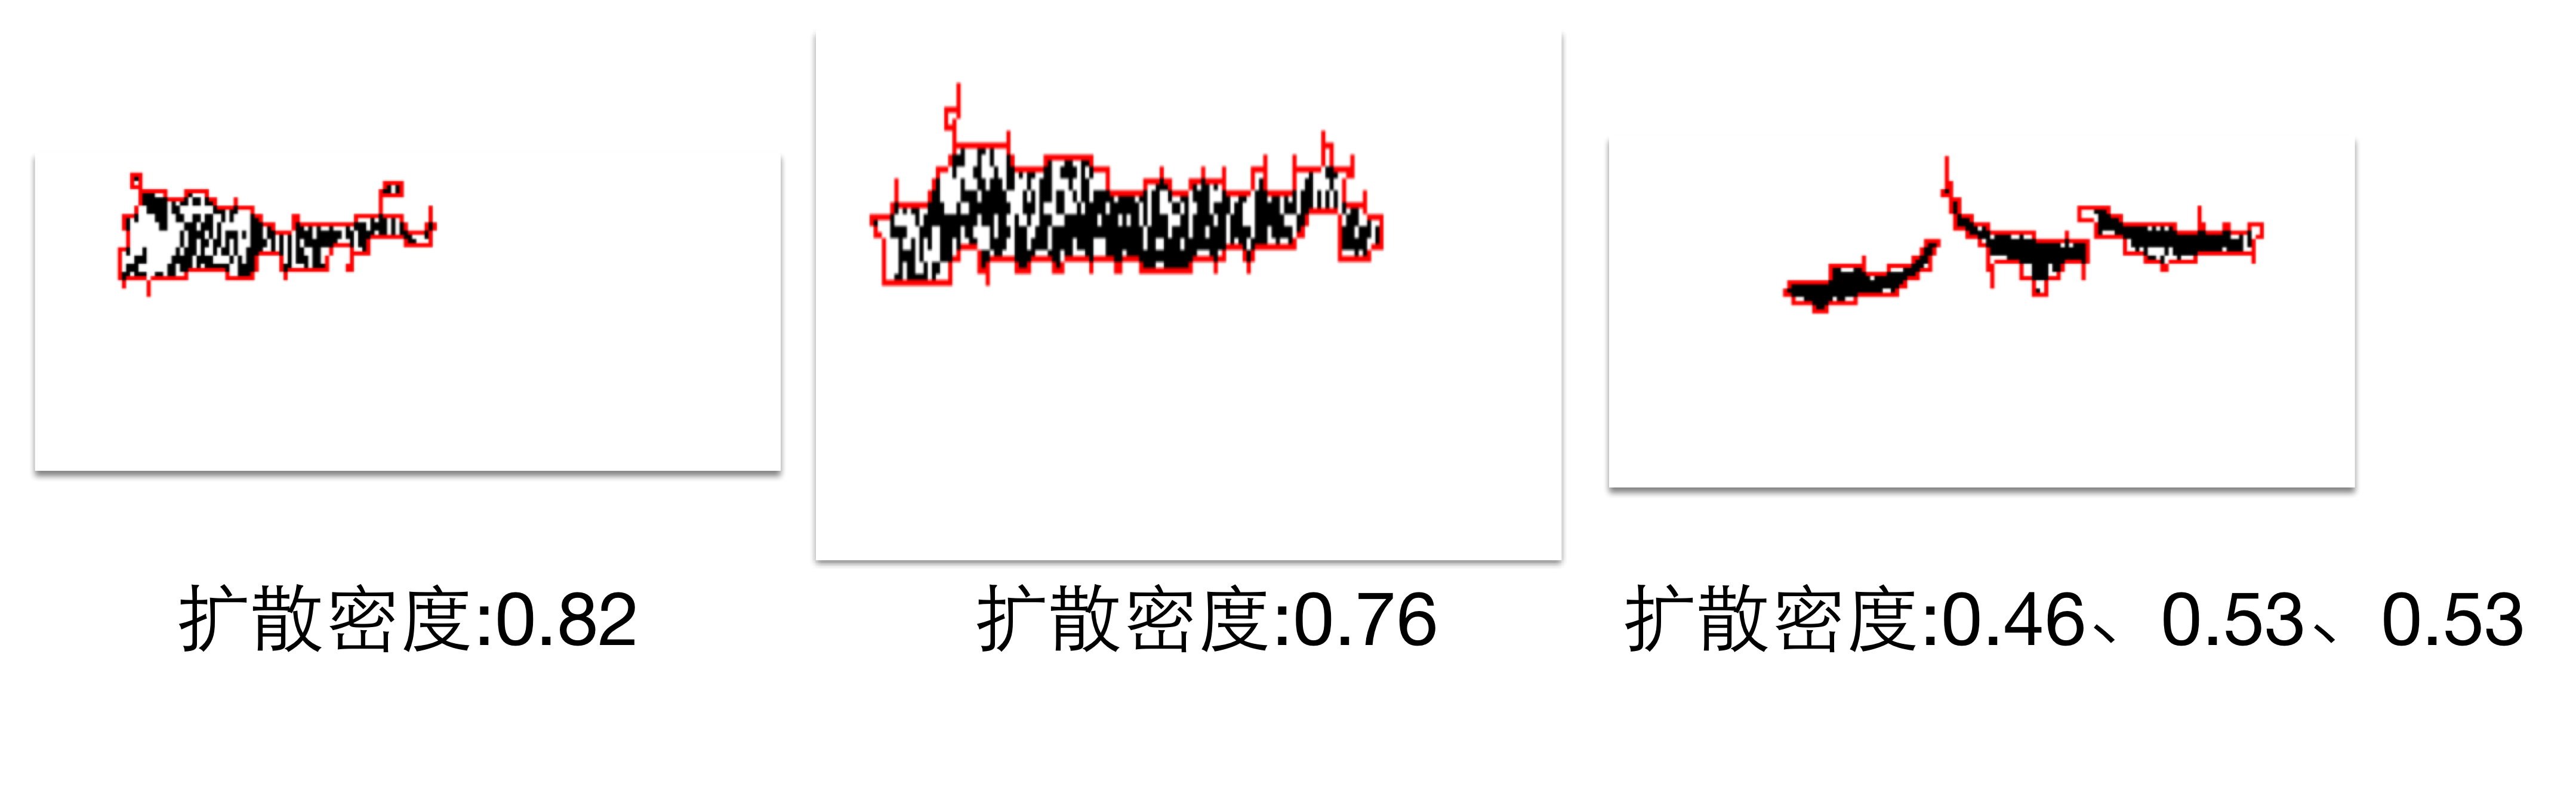
\includegraphics[width=0.7\linewidth]{扩散密度对比.png}

\hspace{-1em}每个描迹区域划分三种(依据$\rho_{area}$、$\rho_{spread}$、$\max{(\rho_{row})}$、$W_{col}$、$N_{nonzero}$)
\begin{enumerate}
\addtolength{\itemindent}{-1em}
\item 常规描迹区域(E层,E2层,Es层l、f、c、h、r、k、n型)
\item 扩散描迹区域(Es层a、s、q型)
\item 直线型(Es层l或f型)与s型混合描迹区域
\end{enumerate}
\end{frame}

\begin{frame}
\frametitle{\ding{204} E区电离图分类}
根据E区所有描迹区域种类再将E区电离图分为五类
\begin{tcolorbox}[colback=blue!5,colframe=blue!75!black]
\begin{itemize}
\vspace{-0.5em}
\addtolength{\itemindent}{-2em}
\item[0] \textcolor{blue}{无描迹电离图}$\Rightarrow$无需度量
\item[1] \textcolor{blue}{常规型电离图}(只包含常规型描迹区域)
\item[2] \textcolor{blue}{扩散型电离图}(只包含扩散型描迹区域)
\item[3] \textcolor{blue}{混合型电离图}(只包含混合型描迹区域)
\item[4] \textcolor{red}{复杂描迹电离图}(包含两种及以上描迹区域)$\Rightarrow$人工度量
\vspace{-1em}
\end{itemize}
\end{tcolorbox}
\end{frame}


\begin{frame}
\frametitle{\ding{205} 描迹分割}
\begin{tcolorbox}[colback=blue!5,colframe=blue!75!black]
\begin{description}
\vspace{-0.5em}
\addtolength{\itemindent}{-4em}
\item[目的] 让分割后的描迹区域内只包含一个E层或Es层描迹。
\item[依据] 区域内描迹的像素分布特点。
\vspace{-0.5em}
\end{description}
\end{tcolorbox}
%\pause
\begin{tcolorbox}[colback=blue!5,colframe=blue!75!black,title=第1类\ 常规型]
\begin{enumerate}
\item 基于虚高的描迹一次分割
\item 基于最高点的描迹二次分割
\item 基于OX波分离的描迹三次分割
\end{enumerate}
\end{tcolorbox}
\begin{columns}
\column{.5\textwidth}
\begin{tcolorbox}[colback=blue!5,colframe=blue!75!black,title=第2类\ 扩散型]
无需进行分割
\end{tcolorbox}
\column{.5\textwidth}
\begin{tcolorbox}[colback=blue!5,colframe=blue!75!black,title=第3类\ 混合型]
描迹区域的密度
\end{tcolorbox}
\end{columns}
\end{frame}


\begin{frame}
\frametitle{\ding{72} 第1类\textbf{常规型}描迹分割}
\centering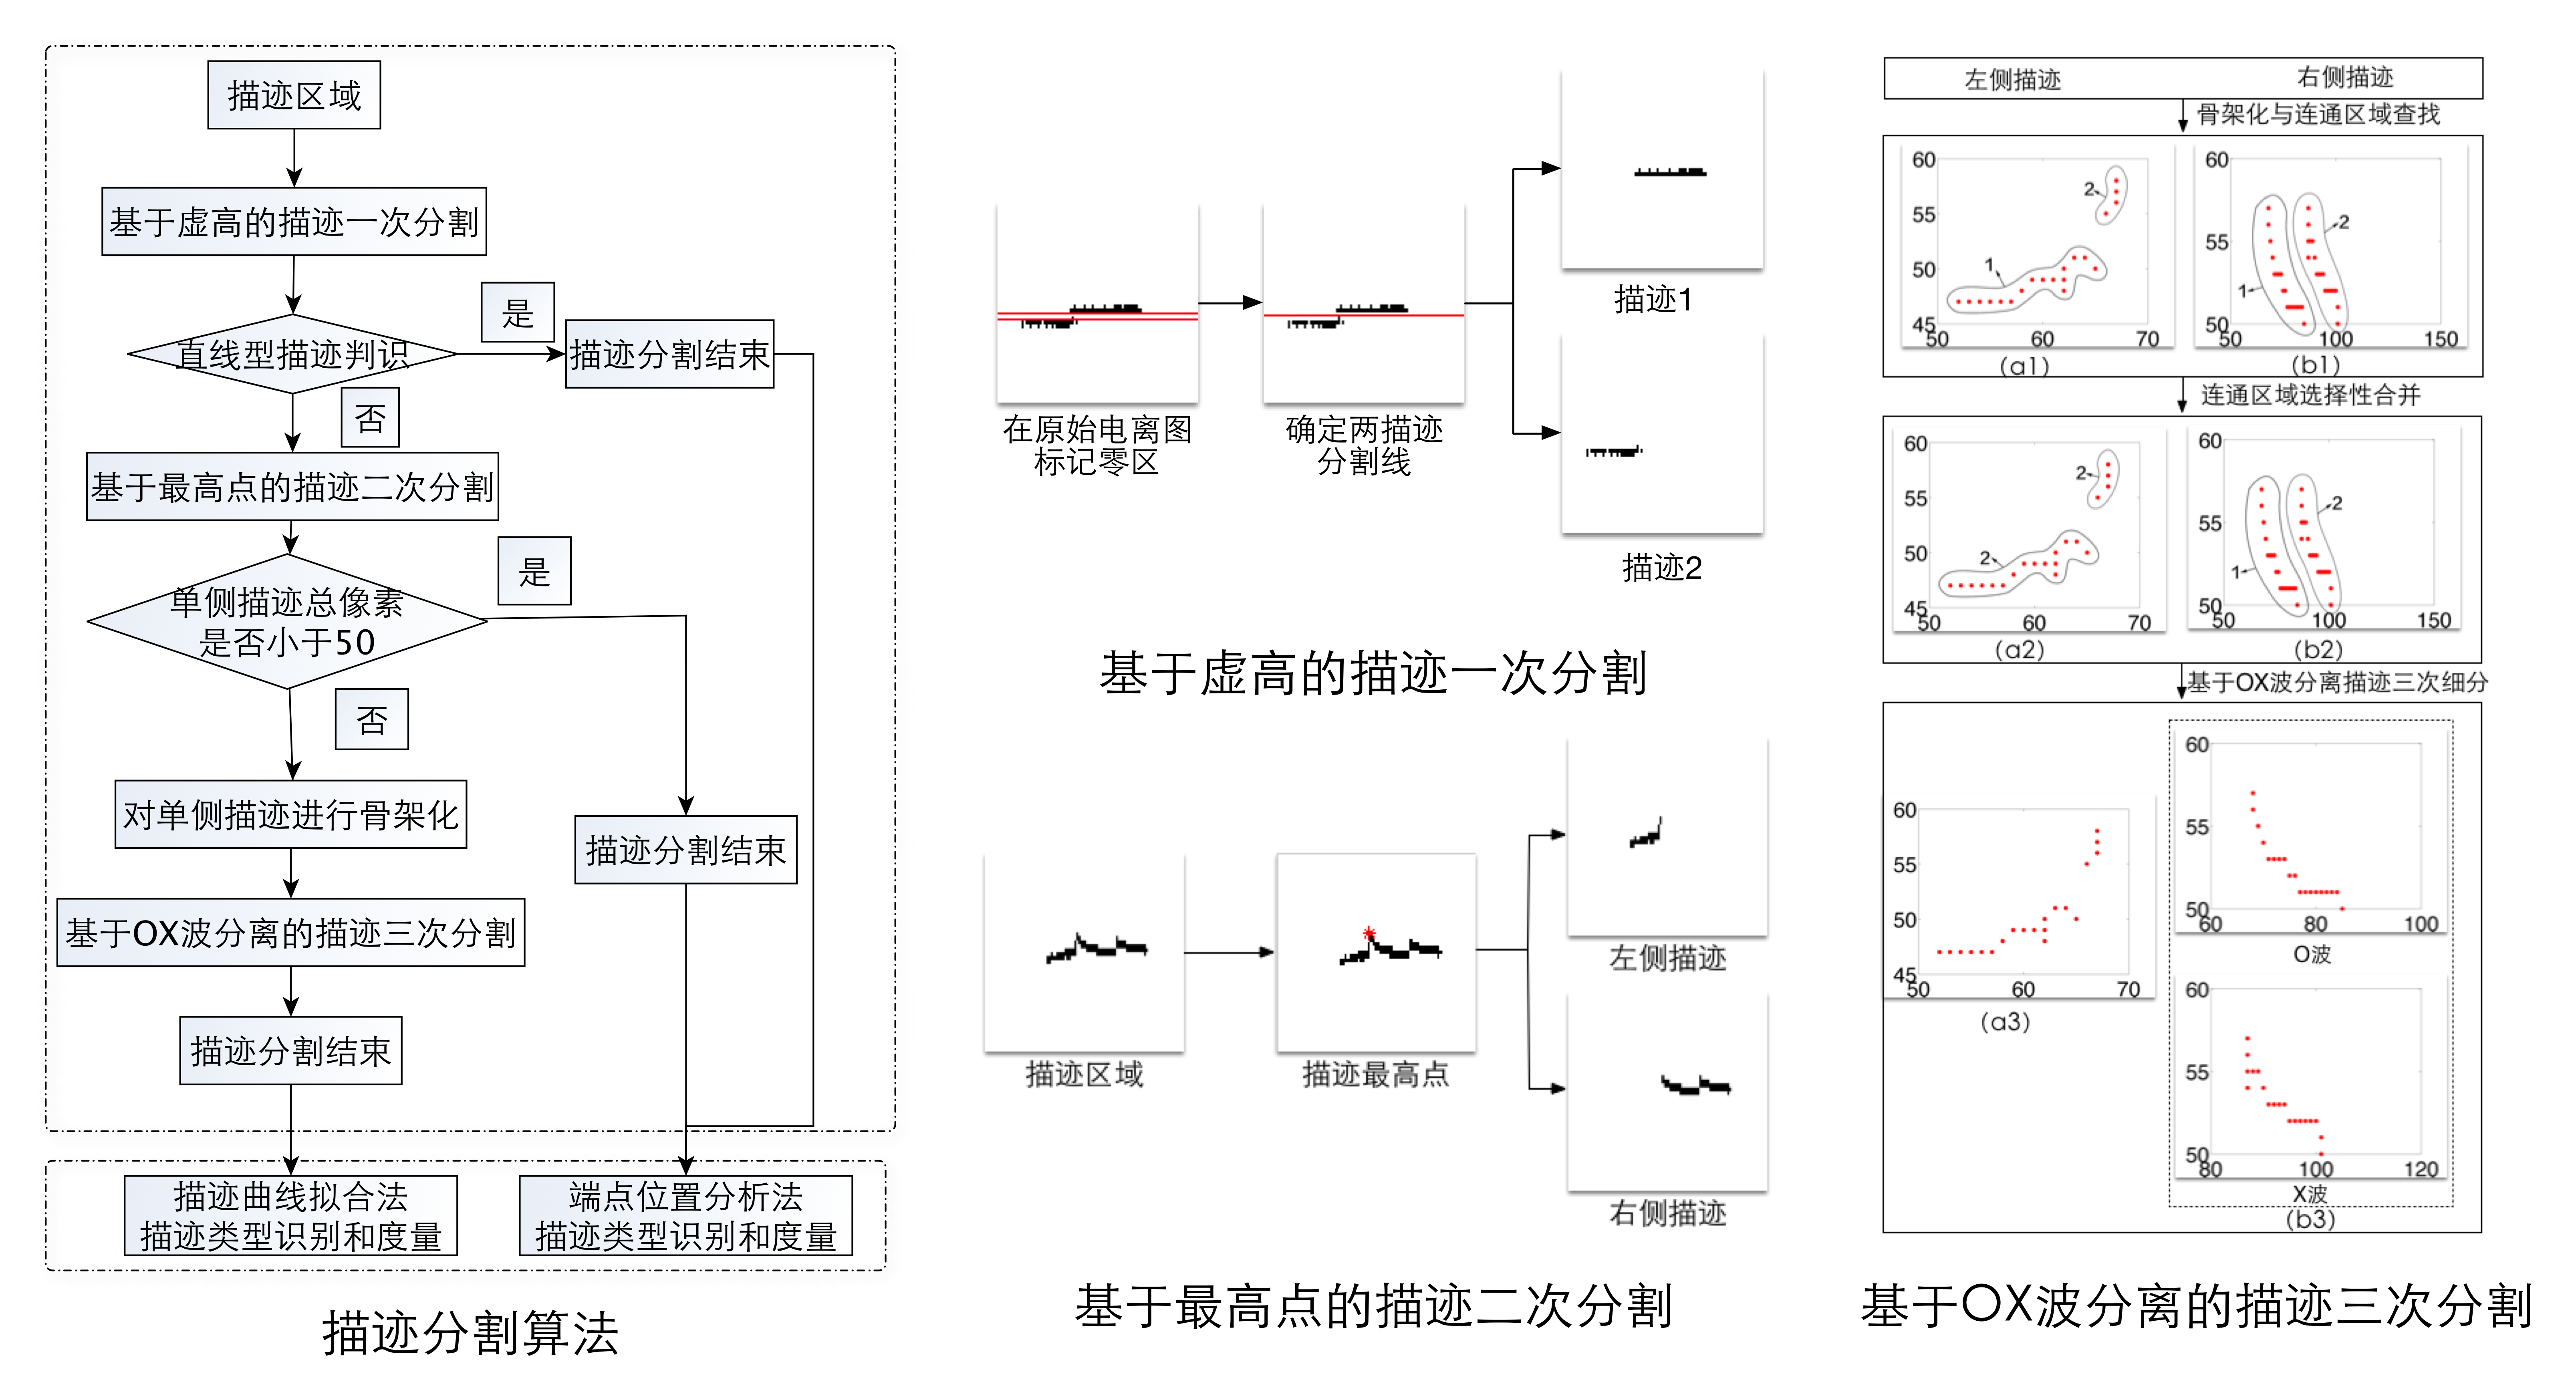
\includegraphics[width=\linewidth]{描迹分割结果.png} 
\end{frame}

\begin{frame}
\frametitle{\ding{72} 第3类\textbf{混合型}描迹分割}
\centering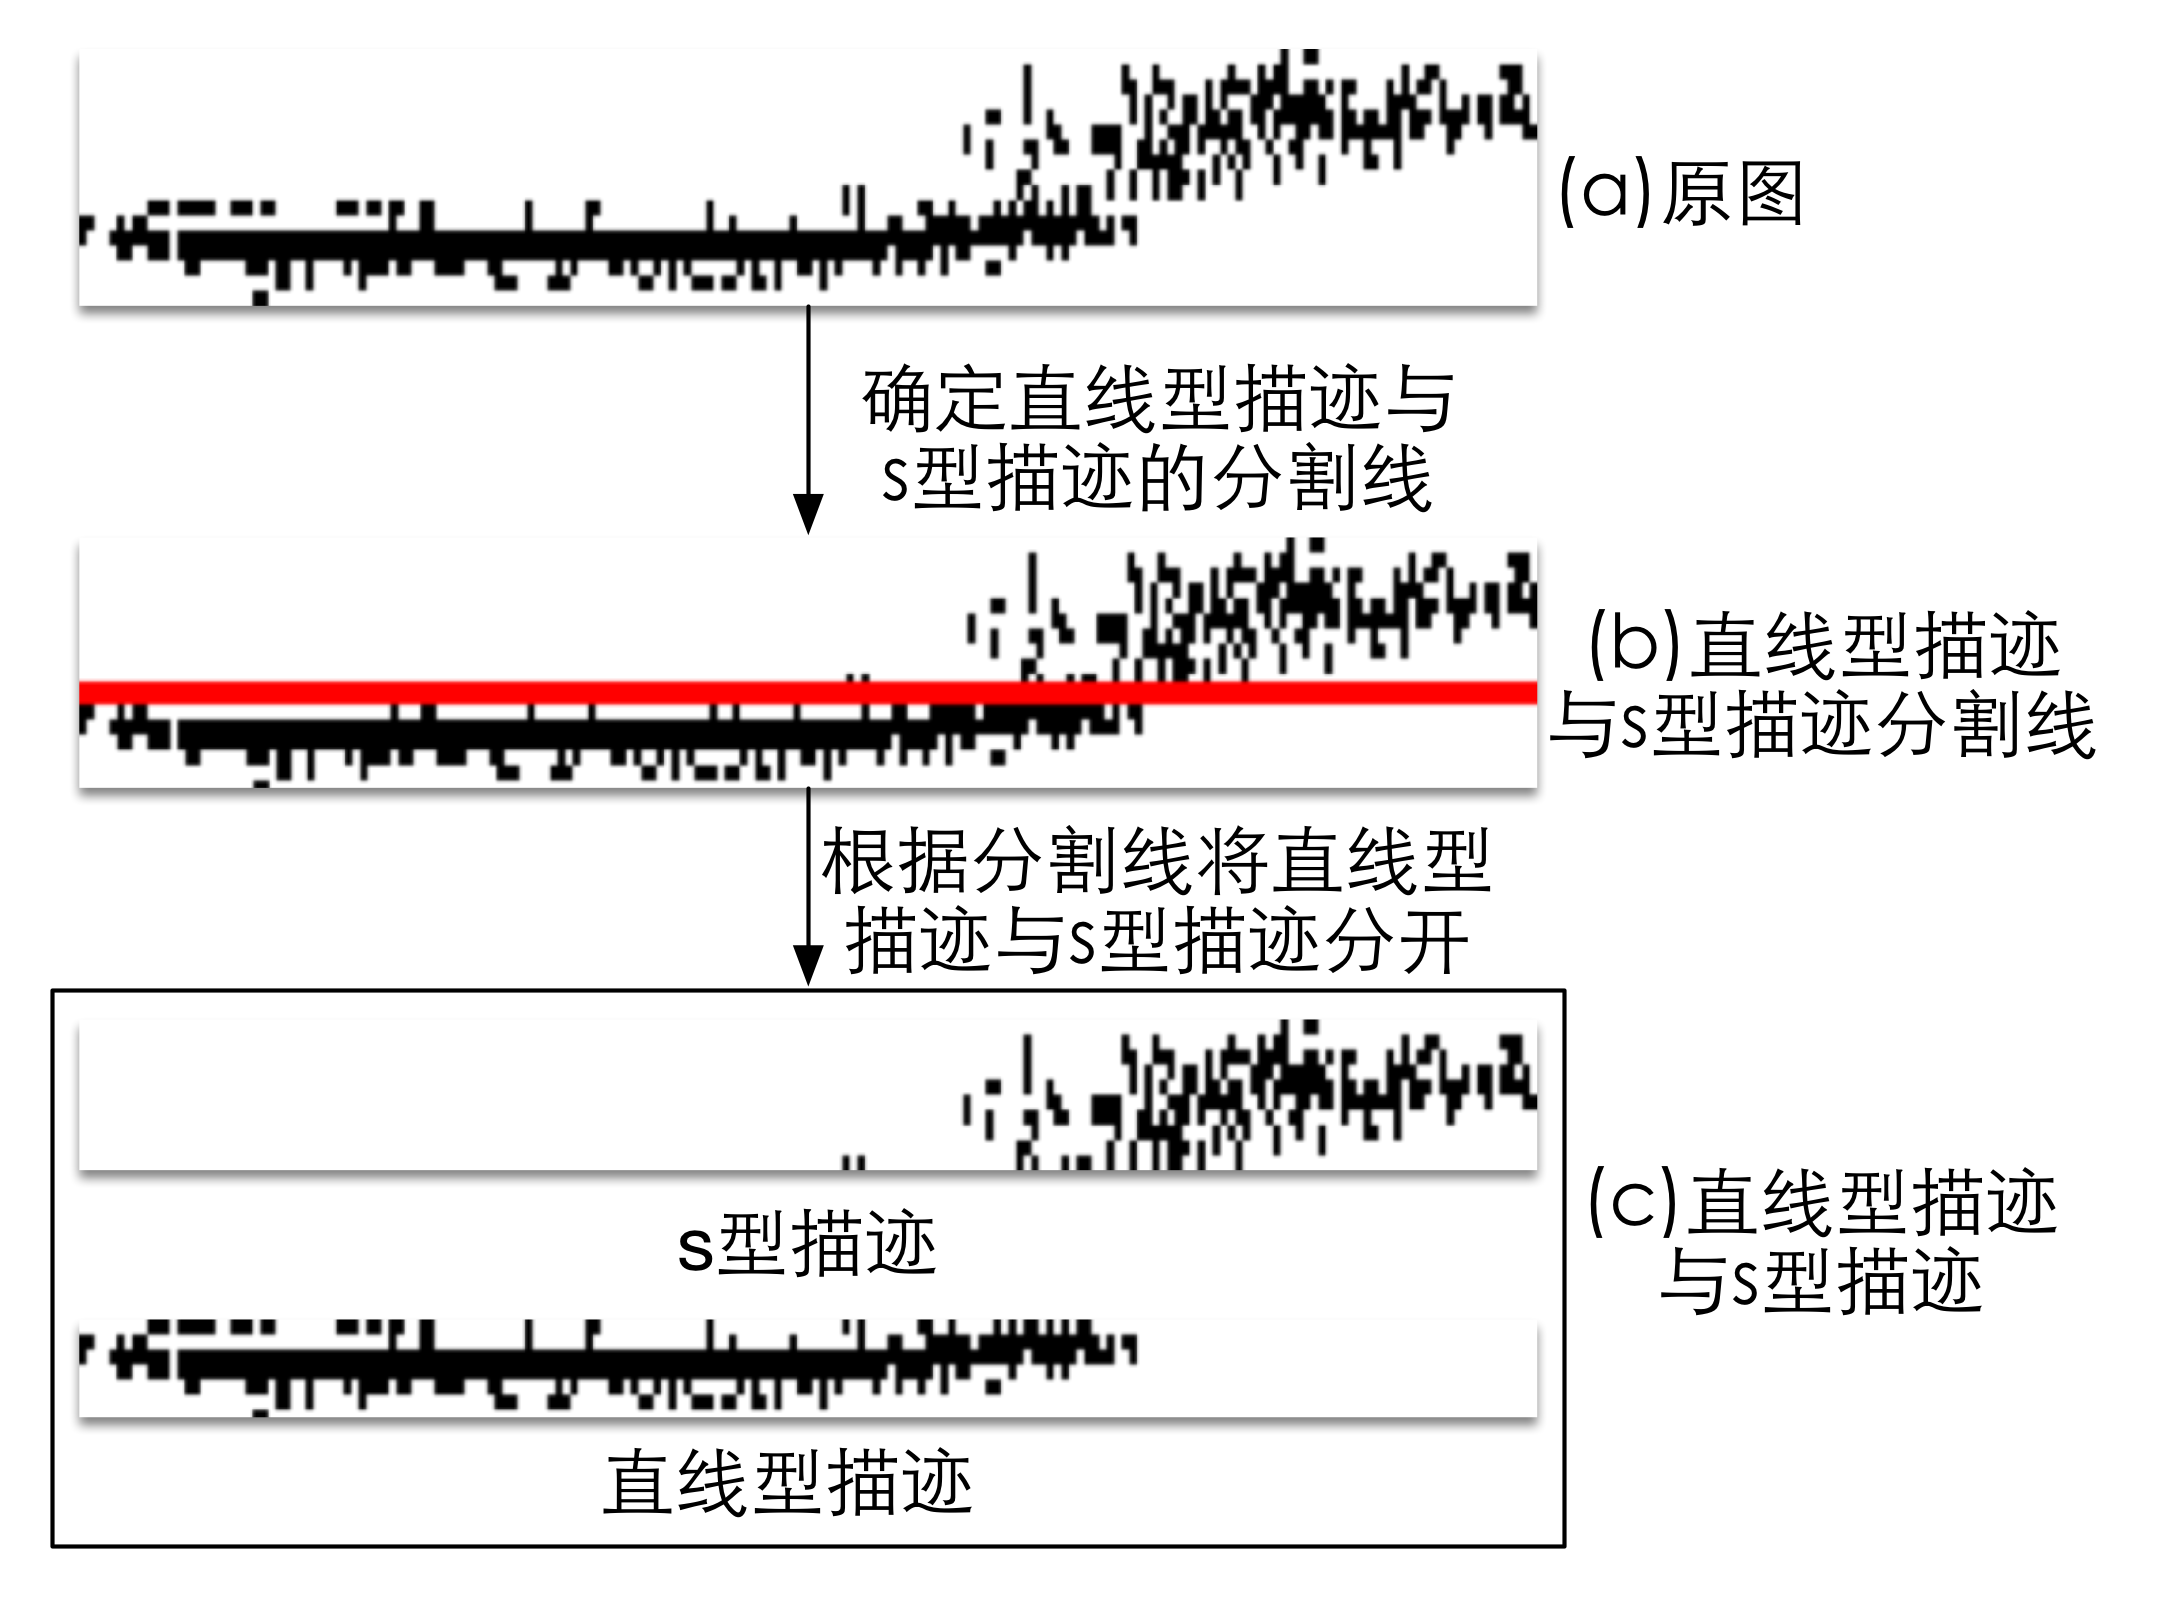
\includegraphics[width=0.8\linewidth]{第2类描迹细分结果.png}
\end{frame}

\begin{frame}
\frametitle{\ding{206} 去除Es层多次反射}
\begin{tcolorbox}[colback=blue!5,colframe=blue!75!black]
\begin{description}
\vspace{-0.2em}
\addtolength{\itemindent}{-4em}
\item[目的] 确定描迹反射次数,有利于准确查找F层描迹
\item[依据] Es层多次反射描迹形成原理。
\vspace{-0.5em}
\end{description}
\end{tcolorbox}
%\pause
\centering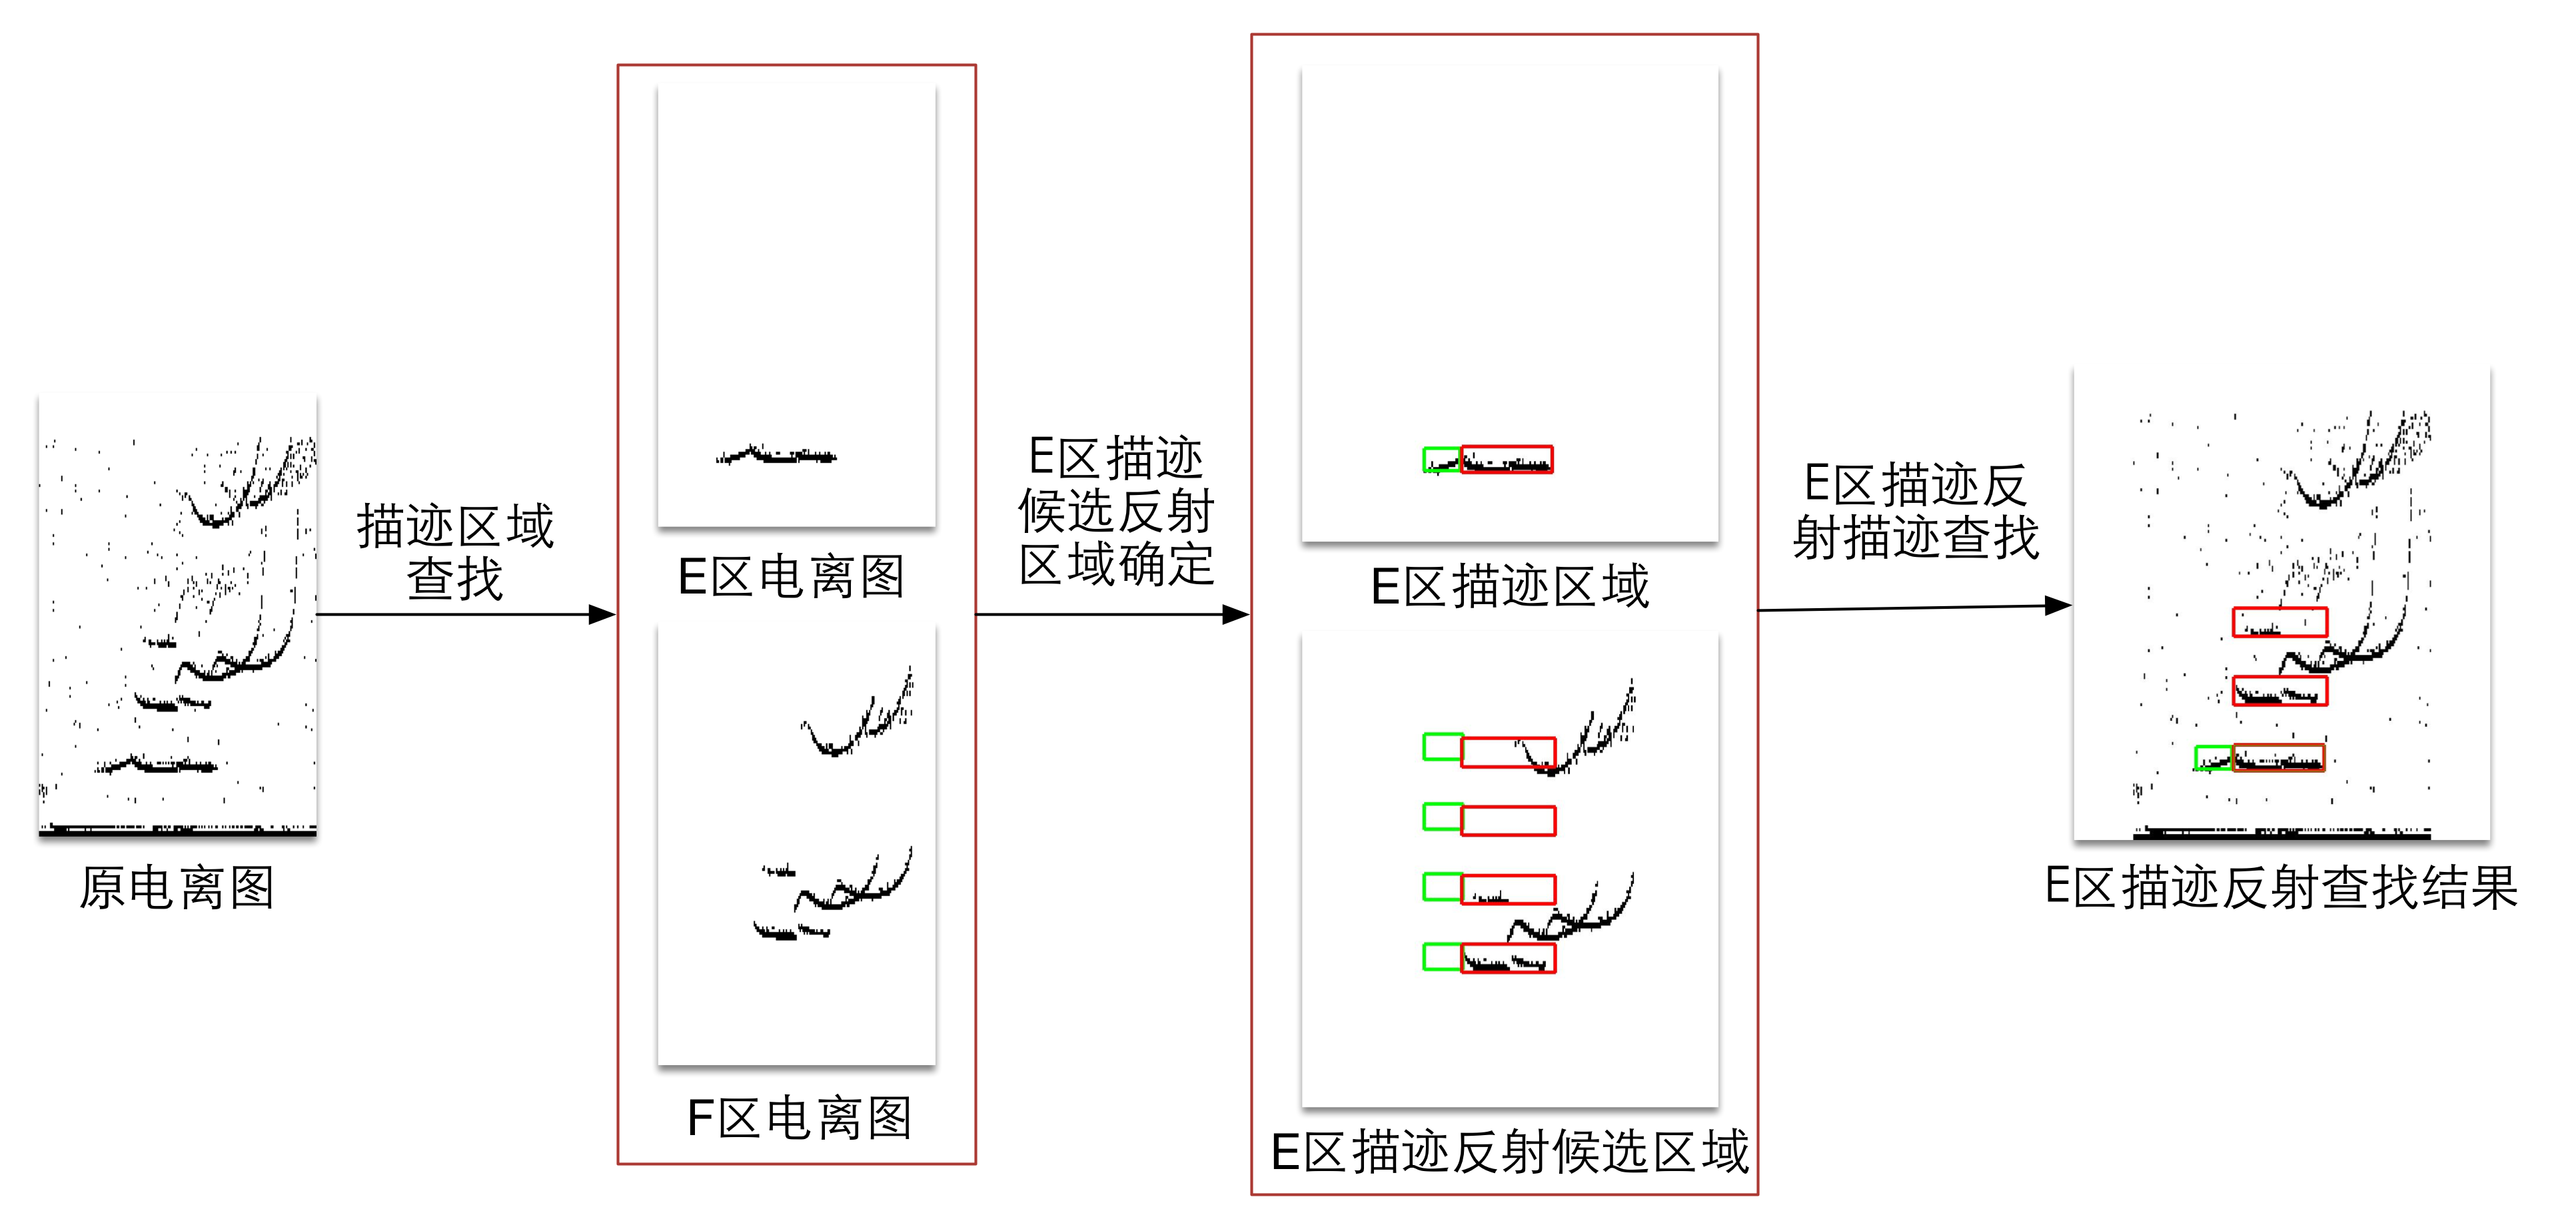
\includegraphics[width=0.9\linewidth]{E区描迹多次反射.png}
\end{frame}

\begin{frame}
\frametitle{\ding{207} E区描迹特征提取}
\begin{tcolorbox}[colback=blue!5,colframe=blue!75!black]
\begin{description}
\vspace{-0.5em}
\addtolength{\itemindent}{-4em}
\item[目的] 识别描迹
\item[依据] 描迹的多样性+人工度量电离图的依据
\vspace{-0.5em}
\end{description}
\end{tcolorbox}
%\pause
\begin{tcolorbox}[colback=blue!5,colframe=blue!75!black,title=常规型描迹]
{\textcolor{blue}{特征:}}电离图的采集时间、 虚高、\textcolor{red}{描迹形状}(上升型、下降型、直线型)、最小频率、最大频率\\
{\textcolor{blue}{提取特征方法:}}端点位置分析法、描迹曲线拟合法


%{\textcolor{blue}{特征:}}电离图的采集时间、 虚高、\textcolor{red}{描迹形状}(上升型、下降型、直线型)、最小频率、最大频率\\
%{\textcolor{blue}{提取特征方法:}}端点位置分析法、描迹曲线拟合法

\end{tcolorbox}
\begin{tcolorbox}[colback=blue!5,colframe=blue!75!black,title=扩散型描迹]

{\textcolor{blue}{特征:}}电离图的采集时间、虚高、描迹区域(长度、宽度)、描迹形状、最小频率、最大频率\\
{\textcolor{blue}{提取特征方法:}}直接提取
\end{tcolorbox}
\end{frame}

\begin{frame}
\frametitle{\ding{208} E区描迹参数自动判读}
\begin{tcolorbox}[colback=blue!5,colframe=blue!75!black]
\begin{description}
\vspace{-0.5em}
\addtolength{\itemindent}{-4em}
\item[目的] 电离层特征参数
\item[依据] 人工度量规则
\vspace{-0.5em}
\end{description}
\end{tcolorbox}
\begin{tcolorbox}[colback=blue!5,colframe=blue!75!black,title=参数判读]
\begin{itemize}
\item 根据描迹特征识别出每个描迹所属的类型。
\item 获取fminF。
\item 参数foE、foEs、hE、hEs、fbEs、Es层描迹类型及反射次数。
\end{itemize}
\end{tcolorbox}
\end{frame}

\begin{frame}
\frametitle{\ding{208} E区描迹参数自动判读}
\centering\includegraphics[width=0.66\linewidth]{201303011045p40s1111改.jpg}
\end{frame}


\section{实验结果与分析}
\begin{frame}
\frametitle{实验结果}
\begin{tcolorbox}[colback=blue!5,colframe=blue!75!black,title=测试数据集]
北京(2013年6月)、新乡(2011年4月)、满洲里(2014年2月)、广州(2013年9月)、昆明(2011年12月)五个地区3576张电离图
\end{tcolorbox}
%\pause
\begin{tcolorbox}[colback=blue!5,colframe=blue!75!black]
\begin{table}[!ht]
\begin{tabular}{|c|c|c|c|c|}
\hline
度量参数(<1MHz)& foE & foEs & fbEs  \\
\hline
判读准确率 & $86.3\%$ & $81.0\%$ & $77.7\%$  \\
\hline
\end{tabular}
\end{table}
\vspace{-1em}
\begin{table}[!ht]
\begin{tabular}{|c|c|c|c|c|}
\hline
度量参数(<10km)& h'Es & h'E \\
\hline
判读准确率& $74.3\%$ & $78.4\%$\\
\hline
\end{tabular}
\vspace{-1em}
\end{table}
\end{tcolorbox}
\begin{tcolorbox}[colback=blue!5,colframe=blue!75!black]
 Es层描迹类型识别准确率为$55.7\%$
\vspace{-1em}
\end{tcolorbox}
\end{frame}


\begin{frame}
\frametitle{结果分析}
 \begin{enumerate}
  \item 本文算法在描迹检测和参数度量方面取得了较好的效果;
  \item 由于人工度量对Es层描迹类型识别存在主观差异,这是导致Es层类型描迹识别准确率低的主要原因。
  \end{enumerate}
  \end{frame}

\section{总结与展望}
\begin{frame}
  \frametitle{总结}
  \begin{enumerate}
  \item 总结了电离图E区描迹人工度量经验;
  \item 提出了电离图E区F区分割算法;
  \item 提出了电离图E区描迹自动判读算法。
  \end{enumerate}
\end{frame}

\begin{frame}
  \frametitle{展望}
  \begin{enumerate}
  \item 对人工度量流程进一步细化;
  \item 将电离层物理模型和物理意义,融入到算法中。
  \end{enumerate}
\end{frame}

%-----------------------------------------------------------------------------------------------------------------------------

%=============================================================================================================================
\begin{frame}
\vspace{2cm}

\centering{\color{blue} \kaishu \Huge{ \emph{\textbf{  谢谢!}}}}\\
\vspace{1.5cm}

\begin{flushright}
\emph{\href{mailto:zhaohongmiao0627@226.com}{\textrm {Xiaoqing~Sun}}}\\
\href{http://www.ouc.edu.cn}{\textrm {Ocean University of China}}\\
\emph{\textrm {2016.05.22}}
\end{flushright}  
\end{frame}

\end{document}
